\section*{Anhang}
\subsection*{Technische Aspekte der Simulation}
\begin{itemize}
	\item Git
	\item Java 8
	\item Maven
	\item Spring
	\item[?] Komplexeres UML
	\item Gebrauchsanweisung
	\item Lizenzen
\end{itemize}
\subsection*{Analysediagramme}
\subsubsection*{Einzelner lernender Fahrer}
\begin{figure}[H]
	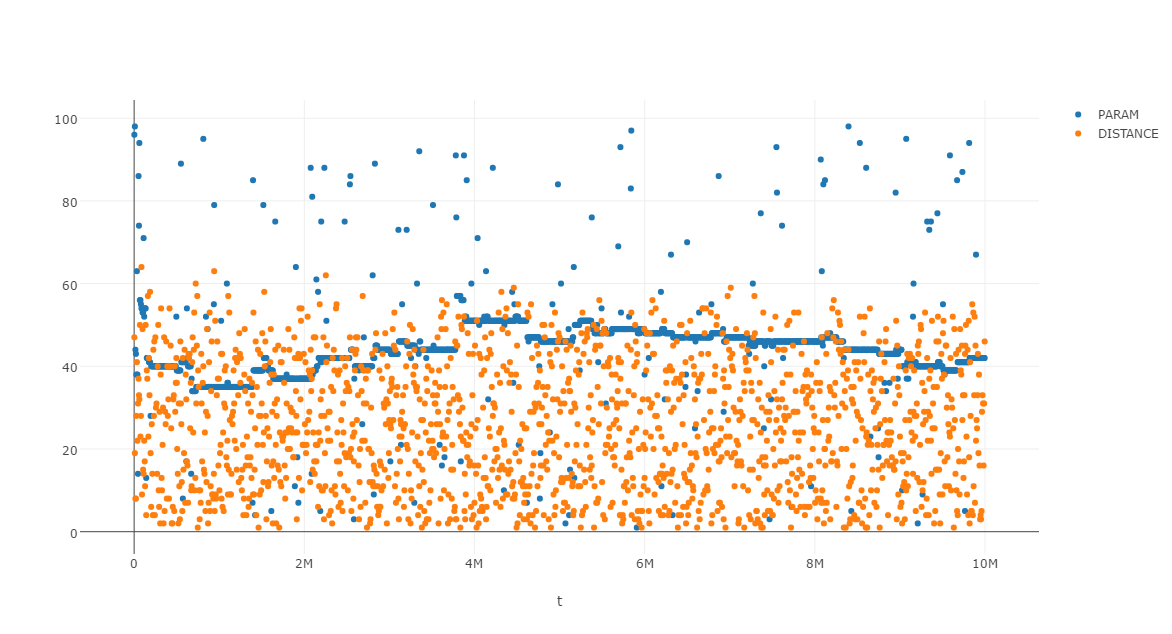
\includegraphics[width=0.8\textwidth]{analyse/SingleMutant/blockcount1.png}
	\caption{\emph{Block-Count}-Heuristik bei 1 Auto pro Minute}\label{fig:ap_sm_bc_1}
\end{figure}
\begin{figure}[H]
	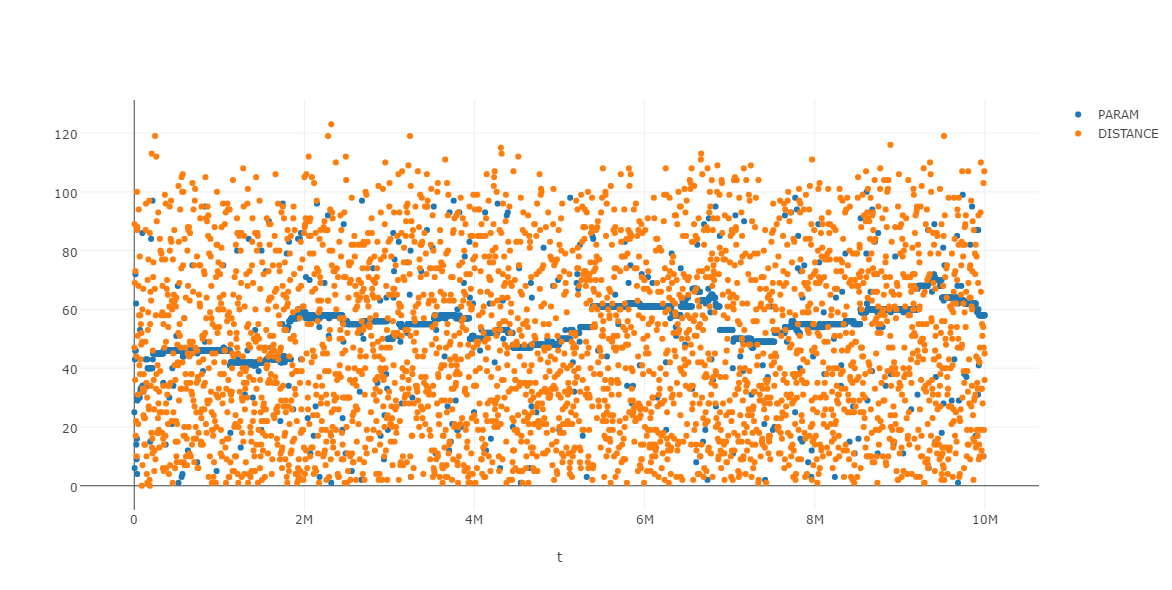
\includegraphics[width=0.8\textwidth]{analyse/SingleMutant/blockcount2.png}
	\caption{\emph{Block-Count}-Heuristik bei 2 Autos pro Minute}\label{fig:ap_sm_bc_2}
\end{figure}
\begin{figure}[H]
	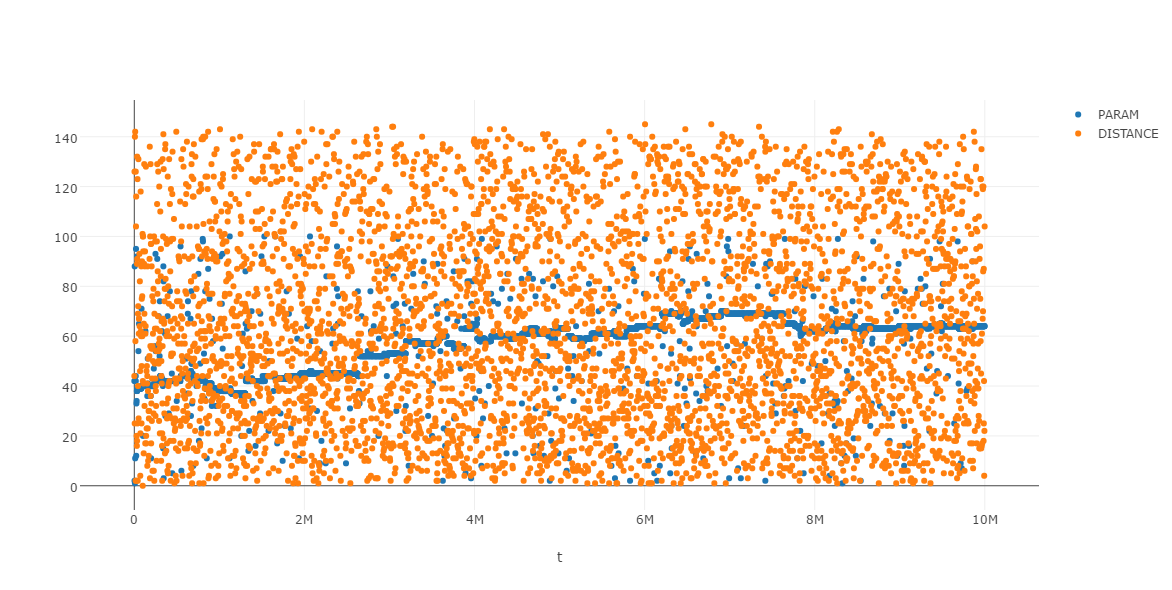
\includegraphics[width=0.8\textwidth]{analyse/SingleMutant/blockcount4.png}
	\caption{\emph{Block-Count}-Heuristik bei 4 Autos pro Minute}\label{fig:ap_sm_bc_4}
\end{figure}
\begin{figure}[H]
	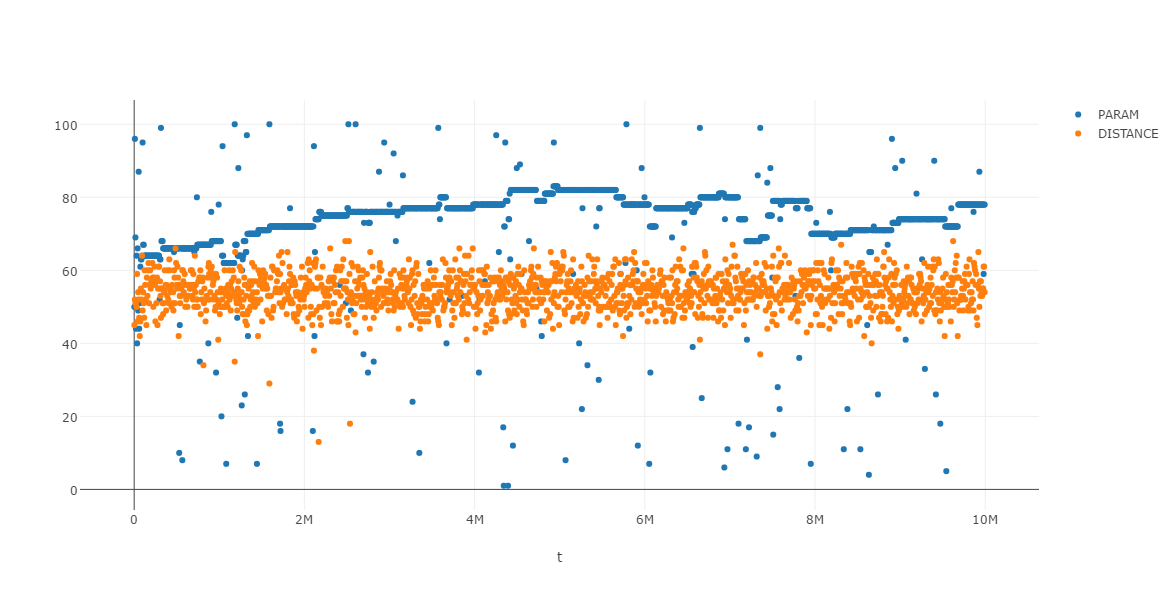
\includegraphics[width=0.8\textwidth]{analyse/SingleMutant/carcount1.png}
	\caption{\emph{Car-Count}-Heuristik bei 1 Auto pro Minute}\label{fig:ap_sm_cc_1}
\end{figure}
\begin{figure}[H]
	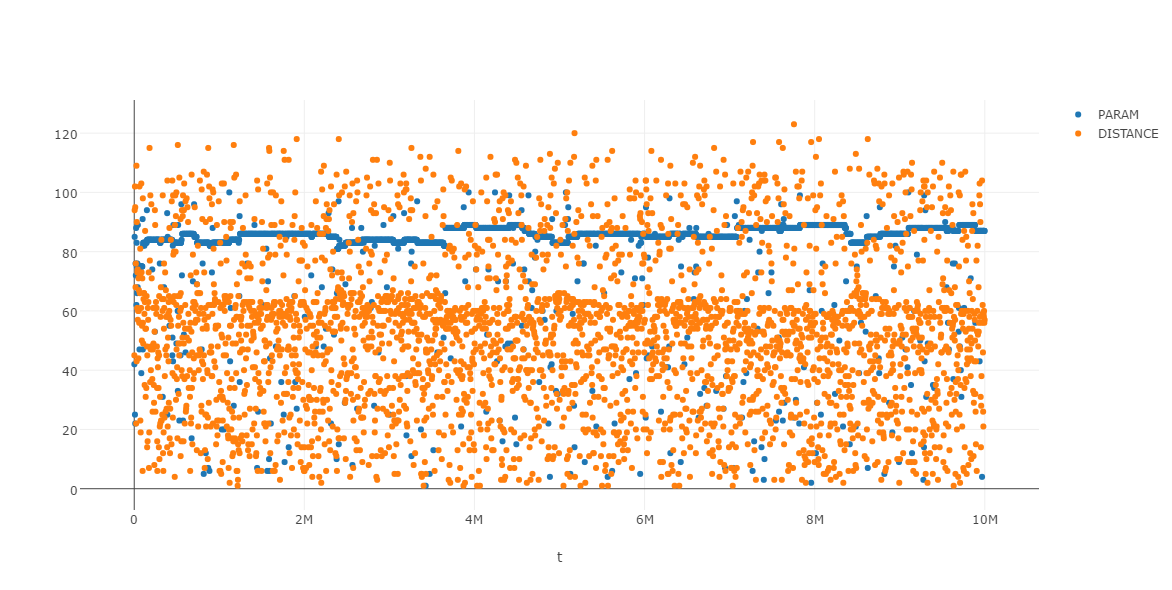
\includegraphics[width=0.8\textwidth]{analyse/SingleMutant/carcount2.png}
	\caption{\emph{Car-Count}-Heuristik bei 2 Autos pro Minute}\label{fig:ap_sm_cc_2}
\end{figure}
\begin{figure}[H]
	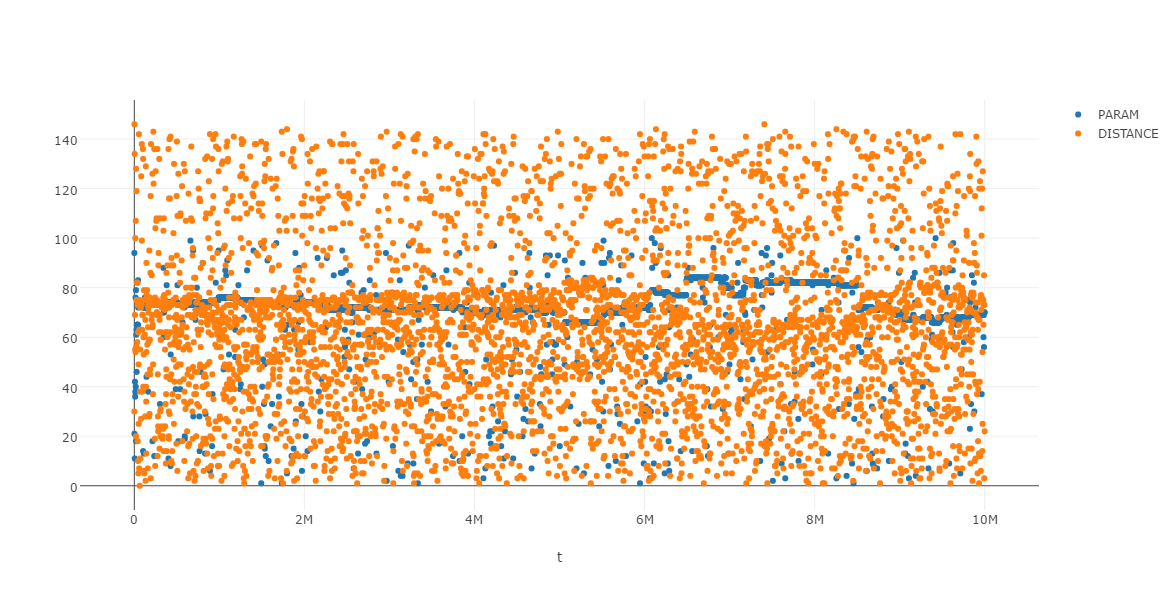
\includegraphics[width=0.8\textwidth]{analyse/SingleMutant/carcount4.png}
	\caption{\emph{Car-Count}-Heuristik bei 4 Autos pro Minute}\label{fig:ap_sm_cc_4}
\end{figure}
\begin{figure}[H]
	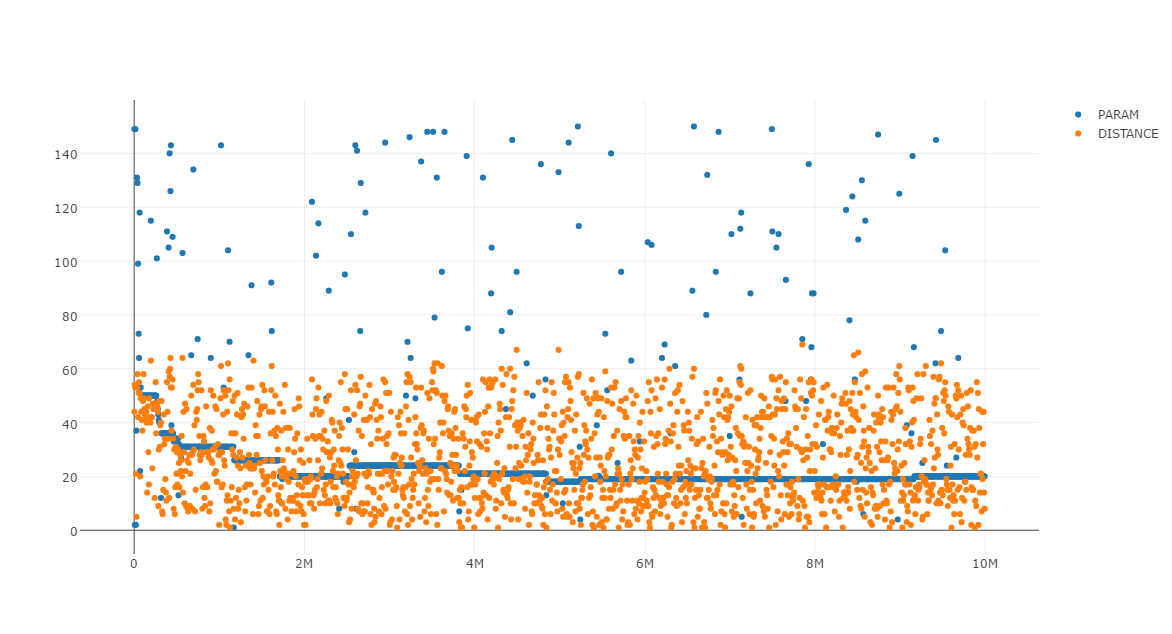
\includegraphics[width=0.8\textwidth]{analyse/SingleMutant/fixeddistance1.png}
	\caption{\emph{Fixed-Distance}-Heuristik bei 1 Auto pro Minute}\label{fig:ap_sm_fd_1}
\end{figure}
\begin{figure}[H]
	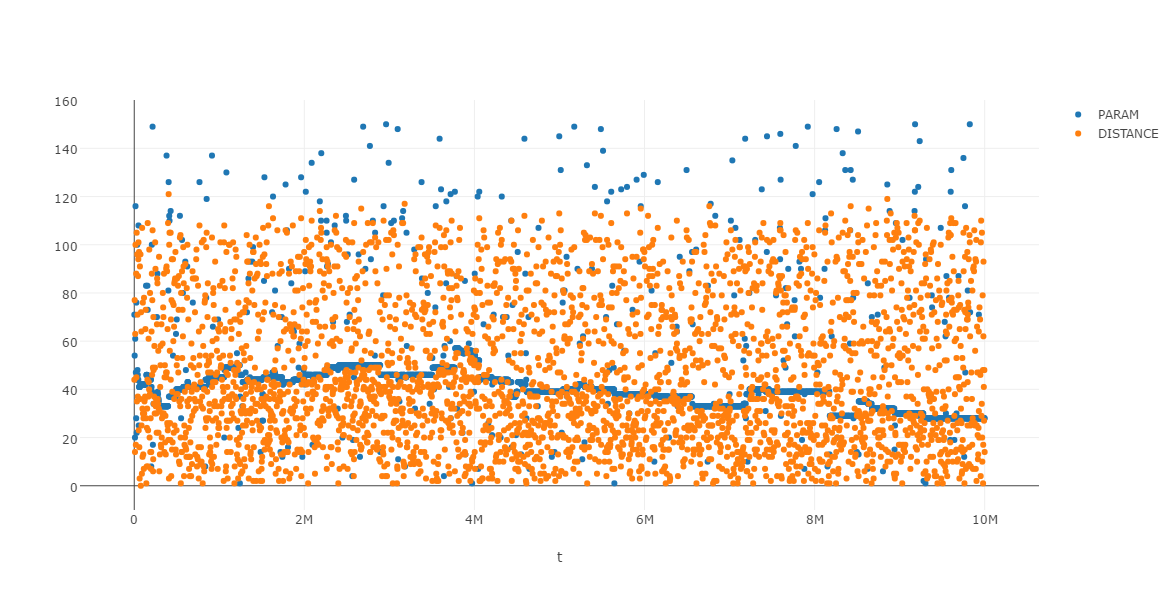
\includegraphics[width=0.8\textwidth]{analyse/SingleMutant/fixeddistance2.png}
	\caption{\emph{Fixed-Distance}-Heuristik bei 2 Autos pro Minute}\label{fig:ap_sm_fd_2}
\end{figure}
\begin{figure}[H]
	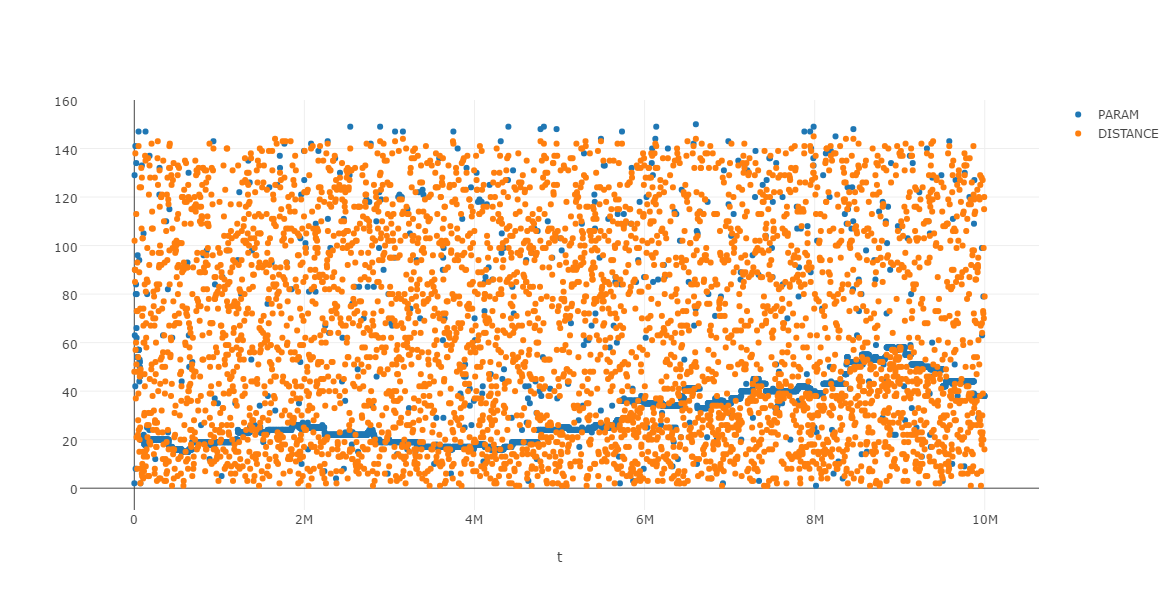
\includegraphics[width=0.8\textwidth]{analyse/SingleMutant/fixeddistance4.png}
	\caption{\emph{Fixed-Distance}-Heuristik bei 4 Autos pro Minute}\label{fig:ap_sm_fd_4}
\end{figure}
\begin{figure}[H]
	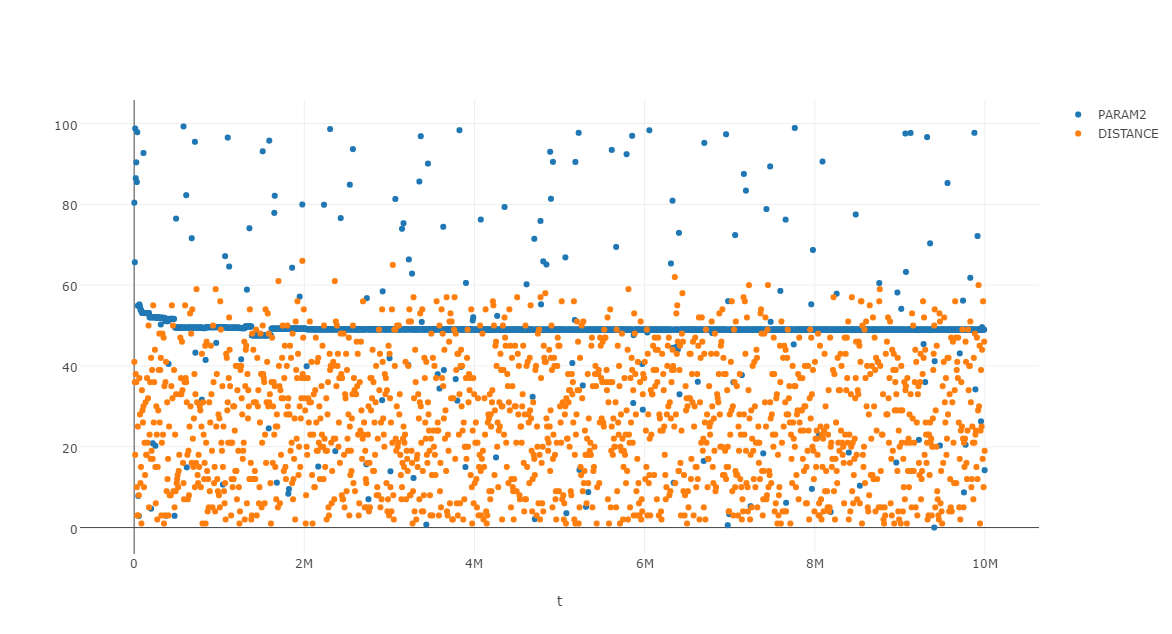
\includegraphics[width=0.8\textwidth]{analyse/SingleMutant/linopzt1.png}
	\caption{Schranke der \emph{Linear-Operator}-Heuristik bei 1 Auto pro Minute}\label{fig:ap_sm_loz_1}
\end{figure}
\begin{figure}[H]
	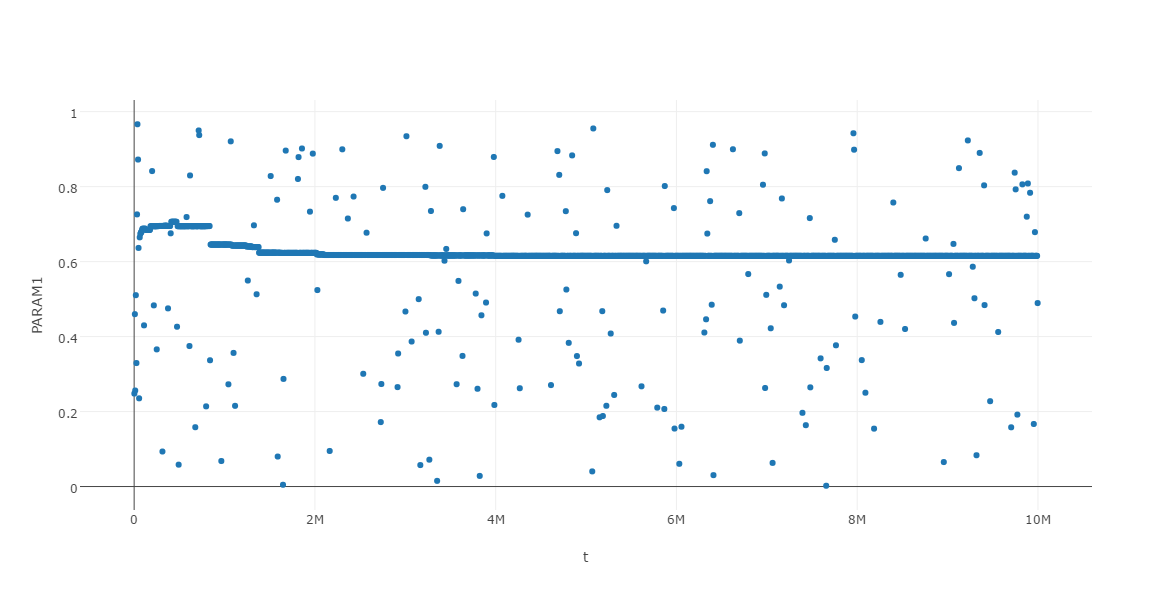
\includegraphics[width=0.8\textwidth]{analyse/SingleMutant/linopa1.png}
	\caption{Geschwindigkeit der \emph{Linear-Operator}-Heuristik bei 1 Auto pro Minute}\label{fig:ap_sm_loa_1}
\end{figure}
\begin{figure}[H]
	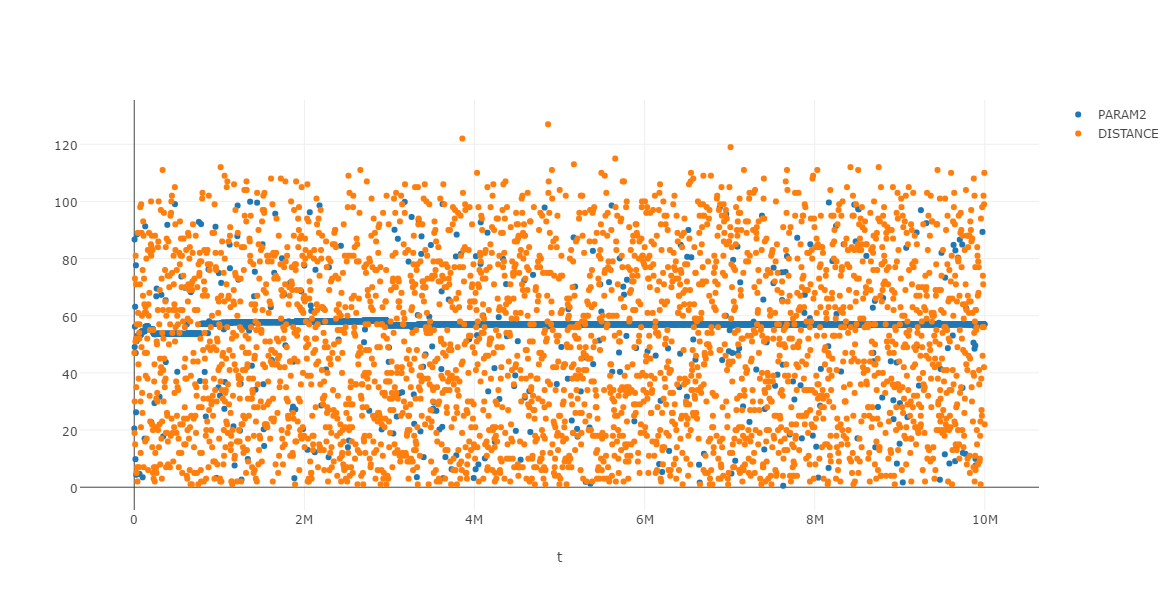
\includegraphics[width=0.8\textwidth]{analyse/SingleMutant/linopzt2.png}
	\caption{Schranke der \emph{Linear-Operator}-Heuristik bei 2 Autos pro Minute}\label{fig:ap_sm_loz_2}
\end{figure}
\begin{figure}[H]
	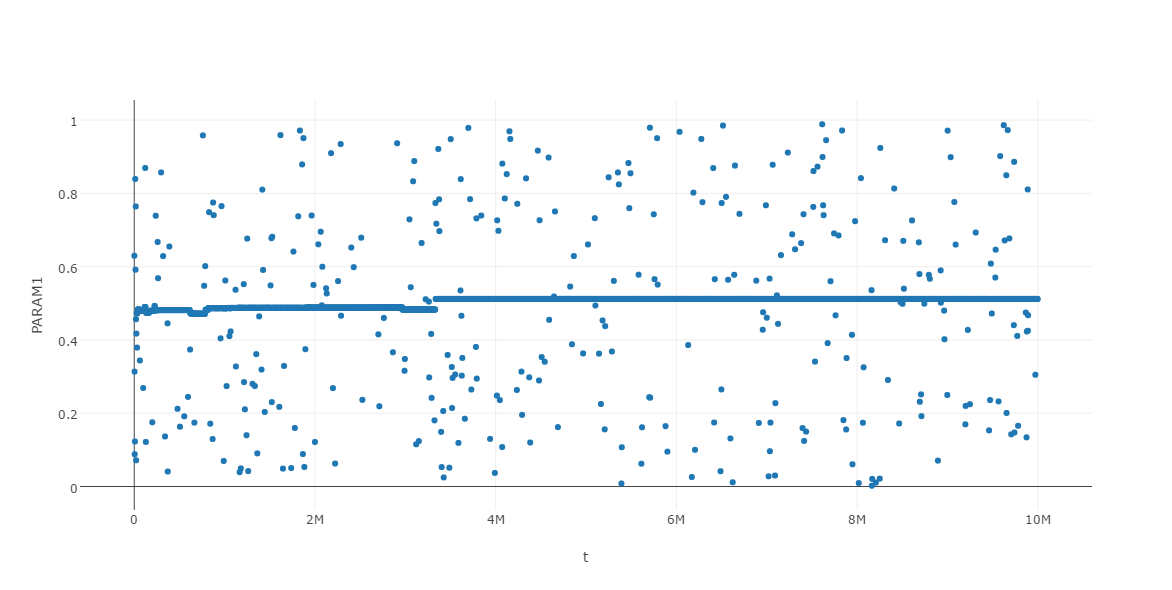
\includegraphics[width=0.8\textwidth]{analyse/SingleMutant/linopa2.png}
	\caption{Geschwindigkeit der \emph{Linear-Operator}-Heuristik bei 2 Autos pro Minute}\label{fig:ap_sm_loa_2}
\end{figure}

\begin{figure}[H]
	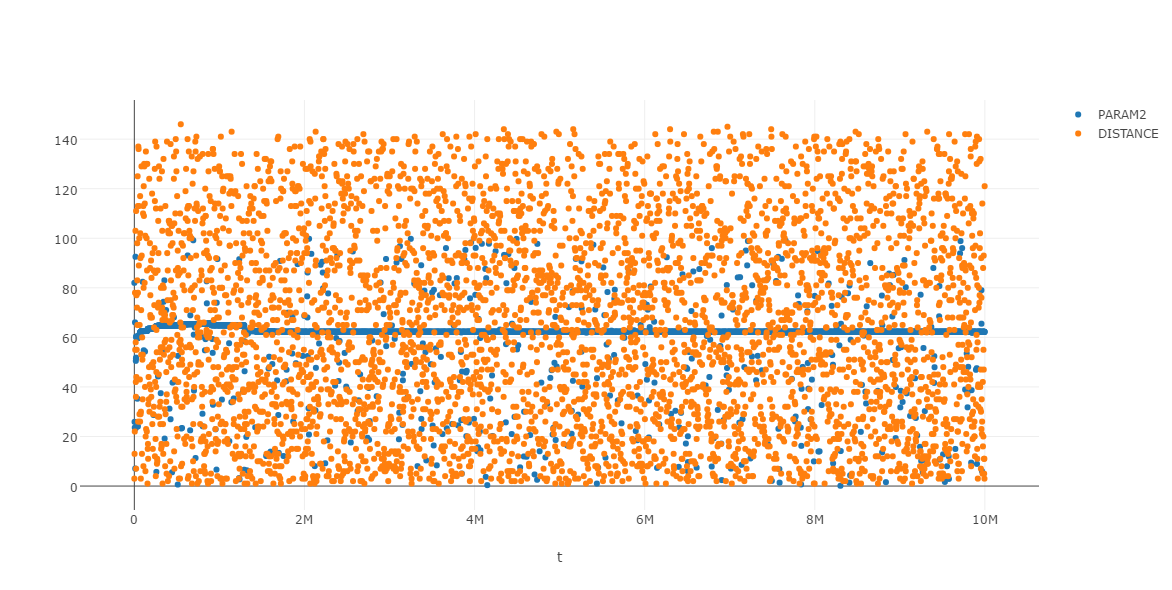
\includegraphics[width=0.8\textwidth]{analyse/SingleMutant/linopzt4.png}
	\caption{Schranke der \emph{Linear-Operator}-Heuristik bei 4 Autos pro Minute}\label{fig:ap_sm_loz_4}
\end{figure}
\begin{figure}[H]
	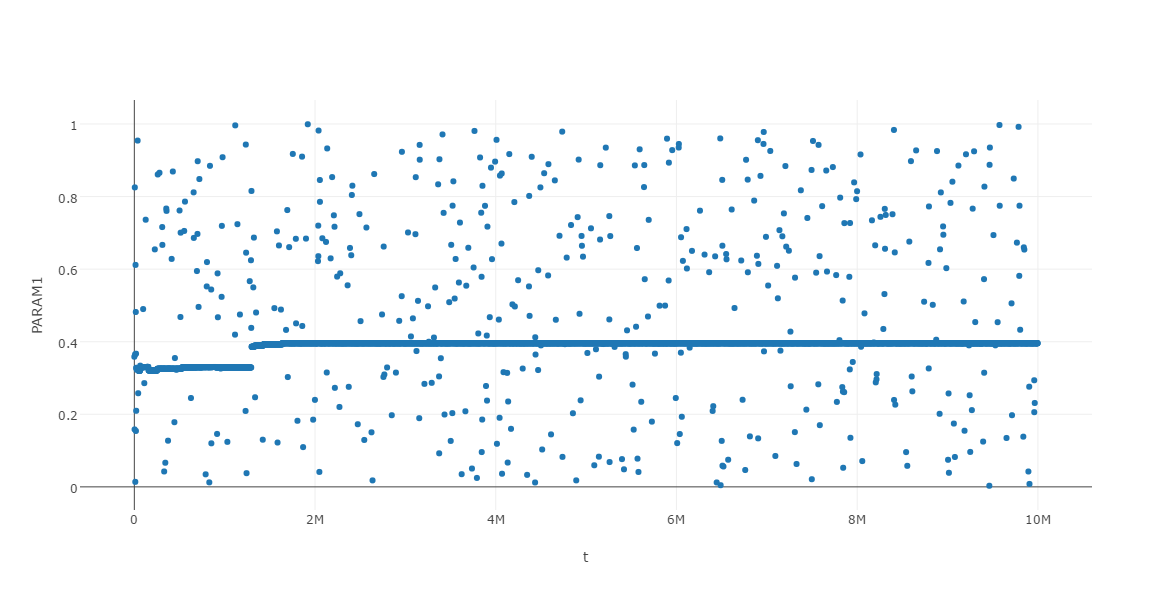
\includegraphics[width=0.8\textwidth]{analyse/SingleMutant/linopa4.png}
	\caption{Geschwindigkeit der \emph{Linear-Operator}-Heuristik bei 4 Autos pro Minute}\label{fig:ap_sm_loa_4}
\end{figure}



\subsubsection*{$20\%$ lernende Fahrer}



\subsubsection*{Nur lernende Fahrer}